\chapter{CONCEPTION}
\begin{spacing}{1.2}
\minitoc
\thispagestyle{MyStyle}
\end{spacing}
\newpage

\section{INTRODUCTION}
\quad Dans cette section, nous nous pencherons sur la conception de notre outil d'annotation, en accordant une attention particulière au développement de l'ontologie. L'ontologie revêt une importance fondamentale au sein de notre système, car elle fournit une structure conceptuelle qui nous permet de représenter et de modéliser les connaissances spécifiques à notre domaine d'étude. Nous détaillerons le processus de création de l'ontologie en décrivant les différentes classes, propriétés et relations utilisées pour dépeindre les entités et les concepts clés. En outre, nous présenterons un processus d'annotation qui tire parti de l'ontologie pour guider et faciliter l'annotation des données en leur attribuant une signification sémantique.\par

\section{Annotation}
Le processus d'annotation est segmenté en plusieurs phases :

\textemdash \textbf{ Acquisition d'images de maniocs }: Cette étape implique la collecte d'images illustrant les différentes affections et la santé des plants de manioc.

\textemdash \textbf{ Prétraitement des images : }Avant d'entamer l'extraction des caractéristiques, il est généralement requis de prétraiter les images afin d'en améliorer la qualité. Cette phase comprend plusieurs opérations visant à optimiser les données visuelles.

\textemdash \textbf{ Extraction des caractéristiques :}À ce stade, des algorithmes spécialisés sont employés pour extraire des informations pertinentes des images, en se fondant sur les divers symptômes associés aux maladies affectant le manioc.

\textemdash \textbf{ Annotation sémantique : }Cette étape implique l'utilisation d'une ontologie pour annoter les caractéristiques extraites. Elle vise à enrichir le processus de détection des maladies et à appliquer des inférences basées sur l'ontologie pour accroître la précision de la détection.

\begin{figure}[htbp]
	\begin{center}
		\begin{minipage}[b]{0.7\textwidth}
			\centering
			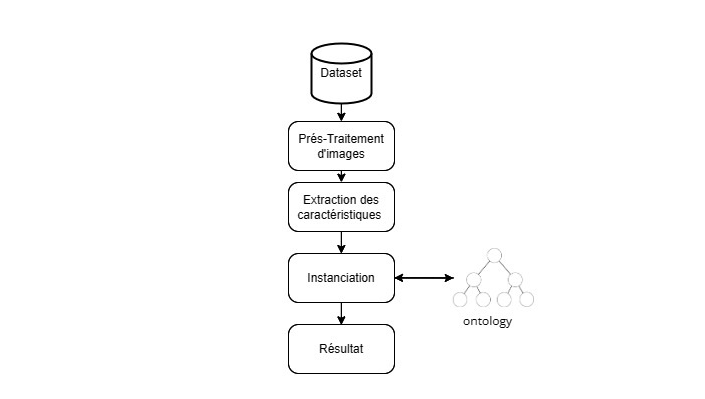
\includegraphics[width=\textwidth]{images/14.png}
			\caption{Illustration d'un processus annotation}
		\end{minipage}
	\end{center}
\end{figure}

\subsection{Mise en place de l'ontologie}
Dans le cadre de l'annotation sémantique, la mise en place d'une ontologie vise principalement à fournir une structure conceptuelle formelle pour représenter et organiser les connaissances spécifiques à un domaine donné. Voici quelques objectifs clés de l'utilisation d'une ontologie dans ce contexte :

\begin{description}
	\item[Structurer les connaissances : ]L'ontologie permet de définir des concepts, des classes, des propriétés et des relations qui représentent les entités et les concepts clés du domaine. Cela offre une structure organisée pour les données annotées, facilitant ainsi la recherche, l'analyse et la compréhension des informations.
	
	\item[Normalisation et standardisation : ]En établissant des termes normalisés et des relations standardisées, une ontologie favorise la cohérence et l'interopérabilité des données annotées. Cela permet aux différents utilisateurs et systèmes de partager et d'échanger efficacement des informations.
	
	\item[Enrichir la sémantique :] L'ontologie attribue une signification explicite aux annotations en définissant des termes et des relations avec précision. Cela permet une compréhension plus approfondie des données et des processus, en offrant un contexte sémantique qui facilite l'interprétation et l'analyse.
	
	\item[Guider le processus d'annotation : ]L'ontologie fournit un cadre de référence pour guider le processus d'annotation en spécifiant les concepts à annoter, les relations à établir et les contraintes à respecter. Cela contribue à assurer la cohérence et la qualité des annotations réalisées par les annotateurs.
	
	\item[Faciliter l'inférence et l'analyse :]En utilisant une ontologie, il est possible d'effectuer des raisonnements basés sur les relations définies entre les concepts. Cela permet d'inférer de nouvelles informations à partir des données annotées, d'identifier des corrélations et des tendances, et d'effectuer des analyses avancées sur les données.
	
	
\end{description}

En résumé, l'objectif principal de la mise en place d'une ontologie dans le cadre de l'annotation sémantique est de fournir un cadre formel et structuré pour représenter, organiser et interpréter les connaissances, ce qui contribue à améliorer la qualité, la cohérence et la valeur des données annotées. \\


\subsection{Collecte d´information (Le Dataset)}
Pour obtenir des informations sur les maladies du manioc, nous avons exploité diverses sources pour recueillir des données précises et fiables. Nous avons examiné des articles scientifiques spécialisés dans le domaine de l'agriculture ainsi que des rapports de recherche [*], [*], [*]. Ces ressources nous ont fourni des détails sur les différentes maladies que trouvons sur chez le manioc, ainsi que sur les symptômes, les causes et les traitements associés à chacune d'entre elles.

\quad Dans cette étude, nous examinons comment utiliser des techniques spéciales pour comprendre et détecter les maladies du manioc à partir d'images des feuilles, des tiges ou des racines infectées.

\quad La culture du manioc est confrontée à diverses menaces, notamment des maladies qui peuvent avoir un impact significatif sur la production et la qualité des récoltes. Parmi les maladies les plus préoccupantes\cite{msikita_lutte_nodate}, on trouve : \\ \\
\textemdash \textbf{  Maladie de la Mosaïque du Manioc, } \\
\textemdash \textbf{ Maladie de la Tache Brune du Manioc, } \\
\textemdash \textbf{ Flétrissement Bactérien du Manioc, } \\
\textemdash \textbf{ Acarien Vert du Manioc, } \\
\textemdash \textbf{  Pourriture des Racines du Manioc, } \\
\textemdash \textbf{ Anthracnose du ManiocAnthracnose du Manioc, } \\
\textemdash \textbf{ Flétrissement Bactérien du Manioc, } \\
\textemdash \textbf{ Maladie Rose du Manioc, } \\
\textemdash \textbf{ Nanisme du Manioc } \\
\textemdash \textbf{ Tache Foliaire du Manioc } \\	
\textemdash \textbf{ Nématode à Nœuds Radiculaires du Manioc } \\	
\textemdash \textbf{ Moucheron Blanc du Manioc } \\	
\textemdash \textbf{ Etc } \\	

Dans cette étude, nous nous concentrerons sur l'analyse sémantique des images pour détecter et comprendre ces maladies spécifiques du manioc. En s'inspirant des images données par notre enseignant, nous mettrons donc l'accent sur : \\ \\
\textemdash \textbf{ Brûlure bactérienne (Bacterial Blight (CBB)), } \\
\textemdash \textbf{ Maladie des stries brunes (Brown Streak Disease (CBSD)), } \\
\textemdash \textbf{ Marbrure verte (Green Mottle (CGM)), } \\
\textemdash \textbf{ Maladie de la mosaïque (Mosaic Disease (CMD)), } \textemdash \textbf{ Et les plantes en bonnes santés. }
\\

Grâce aux images de maladies fournies par notre enseignant, soit plus de 4 000 images,
ainsi qu'à nos recherches sur [*], nous avons réussi à rassembler plus de 20 000 images.

Voyons en détail les maladies sur lesquelles nous avons décidé de baser notre étude.

\paragraph{Brûlure bactérienne (Bacterial Blight (CBB))}
\begin{itemize}
	\item \textbf{Images: }
	\begin{figure}[htbp]
		\centering
		\begin{subfigure}[b]{0.3\textwidth}
			\centering
			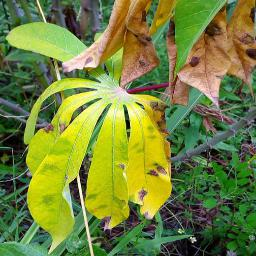
\includegraphics[width=\textwidth]{images/1.jpg}
			\caption{Bactérienne 1}
		\end{subfigure}
		\hfill
		\begin{subfigure}[b]{0.3\textwidth}
			\centering
			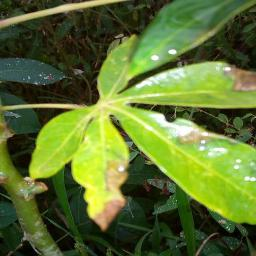
\includegraphics[width=\textwidth]{images/2.jpg}
			\caption{Bactérienne 2}
		\end{subfigure}
		\hfill
		\begin{subfigure}[b]{0.3\textwidth}
			\centering
			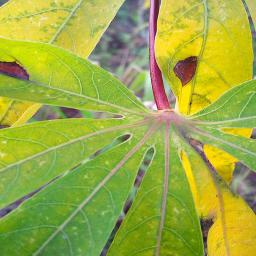
\includegraphics[width=\textwidth]{images/3.jpg}
			\caption{Bactérienne 3}
		\end{subfigure}
		\caption{Images de la brûlure bactérienne}
	\end{figure}
	\item \textbf{Définition: } La brûlure bactérienne est caractérisée par l'apparition de taches nécrotiques, humides et brunes sur les feuilles du manioc. 
	\item \textbf{Cause: } La brûlure bactérienne est une maladie causée par des bactéries qui affectent les plantes, provoquant l'apparition de taches nécrosées sur les feuilles, entraînant souvent le flétrissement, la mort des feuilles et une diminution de la vigueur de la plante.
	\item \textbf{Symptôme: } La bactériose du manioc se présente d'abord sous forme de petites taches humides sur les feuilles, qui deviennent ensuite de plus en plus grandes et brunissent le limbe. Les feuilles touchées finissent par flétrir, mourir et tomber. Ce problème est plus grave pendant la saison des pluies et affecte principalement les jeunes plants.
	\item \textbf{Traitement: } Le traitement de la bactériose du manioc peut impliquer l'utilisation de cultivars résistants, des pratiques culturales appropriées et, parfois, l'application de produits chimiques comme des pesticides.
\end{itemize}

\paragraph{Maladie des stries brunes (Brown Streak Disease (CBSD))}
\begin{itemize}
	\item \textbf{Images: }
	\begin{figure}[htbp]
		\centering
		\begin{subfigure}[b]{0.3\textwidth}
			\centering
			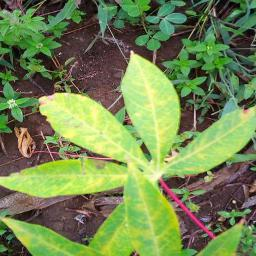
\includegraphics[width=\textwidth]{images/4.jpg}
			\caption{Stries brunes 4}
		\end{subfigure}
		\hfill
		\begin{subfigure}[b]{0.3\textwidth}
			\centering
			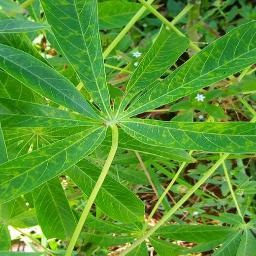
\includegraphics[width=\textwidth]{images/5.jpg}
			\caption{Stries brunes 5}
		\end{subfigure}
		\hfill
		\begin{subfigure}[b]{0.3\textwidth}
			\centering
			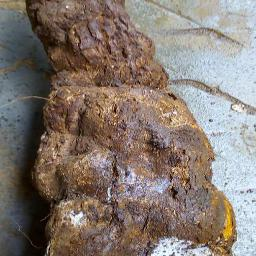
\includegraphics[width=\textwidth]{images/6.jpg}
			\caption{Stries brunes 6}
		\end{subfigure}
		\caption{Images de la maladie des stries brunes}
	\end{figure}
	
	\item \textbf{Définition: } Elle se caractérise par l'apparition de stries brunes sur les racines et les tubercules du manioc infecté, ce qui entraîne une réduction de la qualité et de la quantité des récoltes.
	\item \textbf{Cause: } La Maladie des stries brunes, ou Brown Streak Disease (CBSD), est principalement causée par deux virus du groupe des potyvirus : le virus de la maladie des stries brunes de l'est (BSeMV) et le virus de la maladie des stries brunes de l'ouest (BScMV).
	\item \textbf{Symptôme: } La maladie des stries brunes se manifeste par des symptômes observables sur les feuilles, les tiges et les tubercules du manioc. Sur les feuilles, elle se caractérise par l'apparition de taches jaune-vert, plus prononcées sur les feuilles développées. Contrairement à la mosaïque, les feuilles touchées ne se déforment pas. Sur les tiges, des stries brun foncé ainsi que des lésions nécrotiques peuvent apparaître, principalement sur la partie supérieure verte. Les tubercules peuvent également être déformés, présenter des craquelures et une décoloration.
	\item \textbf{Traitement: } Le traitement de la maladie des stries brunes du manioc peut être difficile car il n'existe pas de méthode curative complètement efficace une fois que la plante est infectée. Cependant, plusieurs approches de gestion peuvent être utilisées pour réduire la propagation de la maladie et limiter ses effets sur les cultures :
	
	\textemdash  Utilisation de cultivars résistants : Sélectionner et cultiver des variétés de manioc qui sont résistantes ou tolérantes à la maladie peut aider à réduire la propagation de la maladie dans les cultures.
	
	\textemdash  Contrôle des vecteurs : La gestion des insectes vecteurs, tels que les pucerons, peut réduire la transmission des virus responsables de la maladie.
	
	\textemdash  Pratiques culturales appropriées : Adopter des pratiques culturales telles que la rotation des cultures, la gestion de l'irrigation et la suppression des plantes infectées peut contribuer à réduire la propagation de la maladie dans les champs.
	
	\textemdash  Utilisation de matériel de plantation sain : Utiliser des boutures de manioc exemptes de maladie pour la plantation peut aider à réduire la propagation de la maladie lors de la multiplication des cultures.
\end{itemize}



\paragraph{Marbrure verte (Green Mottle (CGM))}
\begin{itemize}
	\item \textbf{Images: }
	\begin{figure}[htbp]
		\centering
		\begin{subfigure}[b]{0.3\textwidth}
			\centering
			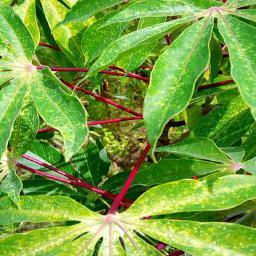
\includegraphics[width=\textwidth]{images/7.jpg}
			\caption{Marbrure verte 7}
		\end{subfigure}
		\hfill
		\begin{subfigure}[b]{0.3\textwidth}
			\centering
			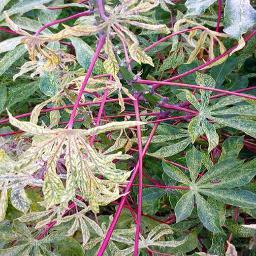
\includegraphics[width=\textwidth]{images/8.jpg}
			\caption{Marbrure verte 8}
		\end{subfigure}
		\hfill
		\begin{subfigure}[b]{0.3\textwidth}
			\centering
			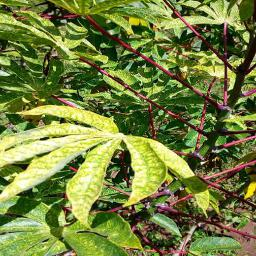
\includegraphics[width=\textwidth]{images/9.jpg}
			\caption{Marbrure verte 9}
		\end{subfigure}
		\caption{Images de la marbrure verte}
	\end{figure}
	
	\item \textbf{Définition: } La Marbrure verte (Green Mottle ou CGM) du manioc se caractérise par l'apparition de marbrures vert clair ou jaune-vert sur les feuilles infectées. Ces marbrures peuvent être irrégulières et s'étendre sur toute la surface des feuilles. Les symptômes sont généralement plus visibles sur la face supérieure des feuilles et peuvent varier en intensité selon le degré d'infection et les conditions environnementales.
	\item \textbf{Cause: } La Marbrure verte (Green Mottle ou CGM) du manioc est principalement causée par une infection virale. Le virus responsable de cette maladie est transmis par des insectes vecteurs, tels que les aleurodes (mouches blanches), qui se nourrissent de la sève des plantes infectées et propagent ainsi le virus à d'autres plantes saines.
	\item \textbf{Symptôme: } Les symptômes de la Marbrure verte (Green Mottle ou CGM) sur les feuilles du manioc se manifestent généralement par l'apparition de marbrures vert clair ou jaune-vert. Ces marbrures peuvent être irrégulières et se propager sur toute la surface des feuilles. Les feuilles affectées peuvent également présenter des déformations et un rabougrissement. Les symptômes peuvent varier en fonction de la gravité de l'infection et des conditions environnementales.
	\item \textbf{Traitement: } Le traitement de la Marbrure verte du manioc (Green Mottle ou CGM) est principalement axé sur la gestion des populations d'insectes vecteurs responsables de la transmission du virus. Voici quelques mesures de gestion qui peuvent être adoptées :
	
	\textemdash  Contrôle des insectes vecteurs : Utilisation de méthodes de lutte intégrée telles que l'utilisation de pièges, de filets anti-insectes et de produits phytosanitaires pour réduire les populations d'insectes vecteurs, comme les aleurodes.
	
	\textemdash  Cultivars résistants : Sélection et plantation de variétés de manioc résistantes ou tolérantes à la maladie, si disponibles.
	
	\textemdash  Rotation des cultures : Pratique consistant à alterner les cultures de manioc avec d'autres cultures non sensibles à la maladie pour réduire la pression des vecteurs et la propagation du virus.
	
	\textemdash  Élimination des plantes infectées : Enlever et détruire les plantes infectées dès l'apparition des symptômes pour réduire la source de l'inoculum viral dans les champs.
\end{itemize}


\paragraph{Maladie de la mosaïque (Mosaic Disease (CMD))}
\begin{itemize}
	\item \textbf{Images: }
	\begin{figure}[htbp]
		\centering
		\begin{subfigure}[b]{0.3\textwidth}
			\centering
			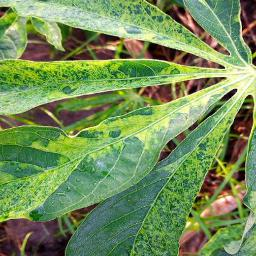
\includegraphics[width=\textwidth]{images/10.jpg}
			\caption{Mosaïque 10}
		\end{subfigure}
		\hfill
		\begin{subfigure}[b]{0.3\textwidth}
			\centering
			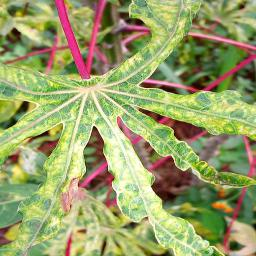
\includegraphics[width=\textwidth]{images/11.jpg}
			\caption{Mosaïque 11}
		\end{subfigure}
		\hfill
		\begin{subfigure}[b]{0.3\textwidth}
			\centering
			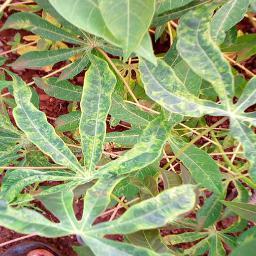
\includegraphics[width=\textwidth]{images/12.jpg}
			\caption{Mosaïque 12}
		\end{subfigure}
		\caption{Images de la maladie de la mosaïque}
	\end{figure}
	
	\item \textbf{Définition: } La Maladie de la mosaïque du manioc se caractérise par l'apparition de motifs de mosaïque sur les feuilles des plants infectés. Ces motifs se présentent sous forme de zones de couleur verte et jaune irrégulières et distinctes.
	\item \textbf{Cause: } La mosaïque du manioc est causée par un virus
	qui s’introduit dans les feuilles et les tiges du
	manioc.
	\item \textbf{Symptôme: } La Maladie de la mosaïque du manioc est principalement causée par des virus, tels que le virus de la mosaïque du manioc (Cassava Mosaic Virus, CMV) et d'autres virus apparentés du groupe des begomovirus. Ces virus sont transmis par des pucerons vecteurs lorsqu'ils se nourrissent de la sève des plantes infectées.
	\item \textbf{Traitement: } Il n'existe pas de traitement curatif pour la Maladie de la mosaïque du manioc une fois que les plantes sont infectées par le virus. Cependant, plusieurs mesures peuvent être prises pour réduire les risques d'infection et limiter les dommages causés par la maladie :
	
	\textemdash  Utilisation de cultivars résistants : Planter des variétés de manioc qui sont génétiquement résistantes ou tolérantes à la Maladie de la mosaïque du manioc peut aider à réduire la propagation de la maladie dans les cultures.
	
	\textemdash  Contrôle des vecteurs : Mettre en place des mesures de contrôle des pucerons vecteurs, tels que l'utilisation de pièges, de filets anti-insectes et de produits phytosanitaires, peut aider à réduire la transmission du virus.
	
	\textemdash  Pratiques culturales appropriées : Adopter des pratiques culturales telles que la rotation des cultures, la gestion de l'irrigation et l'élimination des mauvaises herbes peut contribuer à réduire la pression des vecteurs et la propagation du virus.
\end{itemize}

Quand nous examinons une image de manioc affecté par une maladie, nous remarquons que cette image présente les aspects suivants : la forme, la teinte, la texture et des perforations.
Explorons de manière approfondie ces caractéristiques :

\begin{itemize}
	\item \textbf{ Couleur :} Il s'agit de la teinte ou de la couleur dominante présente dans l'image. La couleur peut fournir des informations sur l'état de santé de la plante, par exemple des taches jaunes ou brunes indiquant une maladie.
	
	\item \textbf{ Contour :} Les contours se réfèrent aux limites et aux formes des objets présents dans l'image. Cela inclut des caractéristiques telles que la surface, le périmètre, la largeur et la hauteur. Les contours peuvent aider à identifier les formes et les structures des feuilles, des racines ou d'autres parties de la plante, permettant ainsi de détecter des anomalies comme des déformations ou des excroissances.
	
	\item \textbf{ Texture :} La texture se réfère aux variations dans la structure de surface de l'image. Cela peut inclure des motifs ou des arrangements de pixels qui indiquent des caractéristiques spécifiques, comme la rugosité ou la douceur des feuilles. Les caractéristiques de texture peuvent aider à diagnostiquer des maladies ou des conditions en analysant des paramètres tels que le contraste, la dissimilarité, l'énergie, l'homogénéité et la corrélation.
	
	\item \textbf{ Symptômes des tiges :} Les symptômes des tiges incluent des signes visibles de maladies ou de stress sur les tiges des plantes. Cela peut inclure la présence de lésions, des déformations, des décolorations ou des changements de texture. Les symptômes peuvent être quantifiés par des mesures telles que la longueur et la largeur des lésions, ainsi que des paramètres de couleur comme la teinte moyenne, la saturation moyenne et la valeur moyenne.
	
	\item \textbf{ Symptômes des feuilles :} Les symptômes des feuilles comprennent les anomalies visibles sur les feuilles, telles que des taches, des décolorations, des trous ou des changements de texture. Ces symptômes peuvent indiquer la présence de maladies, de carences nutritionnelles ou de dommages causés par des ravageurs. Les caractéristiques spécifiques à observer incluent le nombre de taches, la surface des taches, la couleur des taches et la texture des taches.
	
	\item \textbf{ Symptômes des racines :} Les symptômes des racines se manifestent par des changements visibles ou mesurables sur les racines des plantes. Cela peut inclure des déformations, des décolorations, des pourritures ou d'autres anomalies. Les caractéristiques spécifiques à surveiller sont la déformation des racines et la décoloration des racines, qui peuvent indiquer des infections, des carences en nutriments ou d'autres problèmes de santé des plantes.
	
\end{itemize}


\subsection{Conceptualisation}
Dans cette partie, nous explorerons les éléments fondamentaux de la création de l'ontologie, ce qui inclut la clarification des concepts, la détermination des attributs, et la configuration des relations.
\textbf{ Clarification des concepts : } cette phase implique d'établir une liste des concepts identifiés durant la collecte d'informations.

\textbf{ Établir les propriétés : }Cette phase implique la définition des propriétés associées à chaque concept, décrivant ainsi leurs caractéristiques spécifiques. \\

\textbf{ Établir les relations : }Cette étape consiste à établir des liens logiques entre les concepts et les propriétés pour refléter les interrelations entre les différentes entités.

\paragraph{Les propriétés}

\noindent\textbf{Dataset}
\begin{table}[H]
	\centering
	\begin{tabular}{|p{5cm}|p{5cm}|p{5cm}|}
		\hline
		\textbf{Propriété} & \textbf{Domain} & \textbf{Range} \\
		\hline
		hasCreationDate & Dataset & str \\
		\hline
		hasUrl & Dataset & str \\
		\hline
		hasSize & Dataset & str \\
		\hline
		hasAuthor & Dataset & str \\
		\hline
	\end{tabular}
	\caption{Liste des propriétés de Dataset}
\end{table}

\FloatBarrier % Assure que les tableaux sont placés avant de passer à la section suivante

\noindent\textbf{Image}
\begin{table}[H]
	\centering
	\begin{tabular}{|p{5cm}|p{5cm}|p{5cm}|}
		\hline
		\textbf{Propriété} & \textbf{Domain} & \textbf{Range} \\
		\hline
		hasCreationDate & Image & str \\
		\hline
		hasSize & Image & str \\
		\hline
	\end{tabular}
	\caption{Liste des propriétés de l'Image}
\end{table}

\FloatBarrier

\noindent\textbf{Contour}
\begin{table}[H]
	\centering
	\begin{tabular}{|p{5cm}|p{5cm}|p{5cm}|}
		\hline
		\textbf{Propriété} & \textbf{Domain} & \textbf{Range} \\
		\hline
		hasArea & Contour & float \\
		\hline
		hasPerimeter & Contour & float \\
		\hline
		hasWidth & Contour & float \\
		\hline
		hasHeight & Contour & float \\
		\hline
		hasNormalizedArea & Contour & float \\
		\hline
		hasNormalizedPerimeter & Contour & float \\
		\hline
		hasAspectRatio & Contour & float \\
		\hline
	\end{tabular}
	\caption{Liste des propriétés des contours}
\end{table}

\FloatBarrier

\noindent\textbf{Color}
\begin{table}[H]
	\centering
	\begin{tabular}{|p{5cm}|p{5cm}|p{5cm}|}
		\hline
		\textbf{Propriété} & \textbf{Domain} & \textbf{Range} \\
		\hline
		hasHueMean & Contour & float \\
		\hline
		hasHueStd & Contour & float \\
		\hline
		hasSaturationMean & Contour & float \\
		\hline
		hasSaturationStd & Contour & float \\
		\hline
		hasValueMean & Contour & float \\
		\hline
		hasValueStd & Contour & float \\
		\hline
	\end{tabular}
	\caption{Liste des propriétés de la couleur}
\end{table}

\FloatBarrier

\noindent\textbf{Texture}
\begin{table}[H]
	\centering
	\begin{tabular}{|p{5cm}|p{5cm}|p{5cm}|}
		\hline
		\textbf{Propriété} & \textbf{Domain} & \textbf{Range} \\
		\hline
		hasContrast & Texture & float \\
		\hline
		hasDissimilarity & Texture & float \\
		\hline
		hasEnergy & Texture & float \\
		\hline
		hasHomogeneity & Texture & float \\
		\hline
		hasCorrelation & Texture & float \\
		\hline
	\end{tabular}
	\caption{Liste des propriétés de la texture}
\end{table}

\FloatBarrier

\noindent\textbf{RootSymptoms}
\begin{table}[H]
	\centering
	\begin{tabular}{|p{5cm}|p{5cm}|p{5cm}|}
		\hline
		\textbf{Propriété} & \textbf{Domain} & \textbf{Range} \\
		\hline
		hasRootDeformation & RootSymptoms & float \\
		\hline
		hasRootDiscoloration & RootSymptoms & float \\
		\hline
		hasContrast & RootSymptoms & float \\
		\hline
		hasDissimilarity & RootSymptoms & float \\
		\hline
		hasEnergy & RootSymptoms & float \\
		\hline
		hasHomogeneity & RootSymptoms & float \\
		\hline
		hasCorrelation & RootSymptoms & float \\
		\hline
	\end{tabular}
	\caption{Liste des propriétés des symptômes de la racine}
\end{table}

\FloatBarrier

\noindent\textbf{LeafSymptoms}
\begin{table}[H]
	\centering
	\begin{tabular}{|p{5cm}|p{5cm}|p{5cm}|}
		\hline
		\textbf{Propriété} & \textbf{Domain} & \textbf{Range} \\
		\hline
		hasSpotCount & LeafSymptoms & float \\
		\hline
		hasSpotArea & LeafSymptoms & float \\
		\hline
		hasSpotColor & LeafSymptoms & float \\
		\hline
		hasSpotTexture & LeafSymptoms & float \\
		\hline
	\end{tabular}
	\caption{Liste des propriétés des symptômes de la feuille}
\end{table}

\FloatBarrier

\noindent\textbf{StemSymptoms}
\begin{table}[H]
	\centering
	\begin{tabular}{|p{5cm}|p{5cm}|p{5cm}|}
		\hline
		\textbf{Propriété} & \textbf{Domain} & \textbf{Range} \\
		\hline
		hasLesionPresence & StemSymptoms & float \\
		\hline
		hasLesionLength & StemSymptoms & float \\
		\hline
		hasLesionWidth & StemSymptoms & float \\
		\hline
		hasMeanHue & StemSymptoms & float \\
		\hline
		hasMeanSaturation & StemSymptoms & float \\
		\hline
		hasMeanValue & StemSymptoms & float \\
		\hline
	\end{tabular}
	\caption{Liste des propriétés des symptômes de la tige}
\end{table}

\FloatBarrier

\paragraph{Les propriétés}
\noindent\textbf{Relations}
\begin{table}[H]
	\centering
	\begin{tabular}{|p{5cm}|p{5cm}|p{5cm}|}
		\hline
		\textbf{Relation} & \textbf{Domain} & \textbf{Range} \\
		\hline
		hasImage & Dataset & Image \\
		\hline
		hasContour & Image & Contour \\
		\hline
		hasTexture & Image & Texture \\
		\hline
		hasRootSymptoms & Image & RootSymptoms \\
		\hline
		hasLeafSymptoms & Image & LeafSymptoms \\
		\hline
		hasStemSymptoms & Image & StemSymptoms \\
		\hline
	\end{tabular}
	\caption{Liste des relations}
\end{table}

\FloatBarrier

\subsection{Extraction des caractéristiques}
Dans notre contexte nous allons baser sur les descripteurs suivants :

\subsubsection{Les descripteurs de couleur}
Dans le contexte de l'analyse sémantique des maladies du manioc, les descripteurs de couleur jouent un rôle crucial. Ils permettent une évaluation précise et objective des variations de couleur des feuilles de manioc, facilitant ainsi la détection précoce des maladies et la prise de décisions appropriées pour la gestion des cultures.

Pour simplifier cette analyse, les images des feuilles de manioc sont converties dans l'espace de couleur HSV (Teinte, Saturation, Valeur). Cette transformation offre une représentation significative des informations colorimétriques, permettant la réalisation d'opérations de seuillage et de filtrage précises, ainsi que la détection d'anomalies basée sur la teinte.

Dans l'espace de couleur HSV, chaque pixel est caractérisé par trois composantes : la teinte, la saturation et la valeur. La teinte représente la couleur dominante de chaque pixel, la saturation indique son intensité, tandis que la valeur correspond à sa luminosité ou sa brillance. Cette représentation facilite grandement l'analyse des symptômes des maladies, tels que les taches, les décolorations ou les anomalies de pigmentation, sur les feuilles de manioc.

Le processus d'extraction des caractéristiques de couleur peut être réalisé à l'aide d'outils informatiques tels que OpenCV, qui permettent de calculer des statistiques telles que la moyenne et l'écart type de la teinte, de la saturation et de la valeur des pixels dans les images. Ces caractéristiques fournissent des informations essentielles pour évaluer l'état de santé des plantes et détecter la présence de maladies.

Voici les formules mathématiques pour la moyenne et l'écart type : 

La formule de la moyenne :
\[
\mu = \frac{1}{N} \sum_{i=1}^{N} x_i
\]
Où \( \mu \) représente la moyenne, \( N \) est le nombre d'échantillons et \( x_i \) est la valeur de l'échantillon \( i \).

La formule de l'écart type :
\[
\sigma = \sqrt{\frac{1}{N} \sum_{i=1}^{N} (x_i - \mu)^2}
\]
Où \( \sigma \) représente l'écart type, \( N \) est le nombre d'échantillons, \( x_i \) est la valeur de l'échantillon \( i \), et \( \mu \) est la moyenne.

\subsubsection{Descripteur de Contour}
Le descripteur de contour est un outil essentiel dans l'analyse d'images pour caractériser la forme des objets identifiés. Il permet de quantifier les propriétés géométriques des contours des objets présents dans une image.

Le processus de calcul des caractéristiques de contour implique plusieurs étapes :

\begin{enumerate}
	\item \textbf{Conversion en Niveaux de Gris} : L'image originale est convertie en niveaux de gris pour simplifier le traitement et l'analyse ultérieure.
	
	\item \textbf{Seuillage} : Une technique de seuillage est appliquée pour binariser l'image et segmenter les objets d'intérêt du fond.
	
	\item \textbf{Détection de Contours} : Les contours des objets binarisés sont détectés à l'aide d'algorithmes de détection de contours tels que l'algorithme de détection de contour de Canny.
	
	\item \textbf{Calcul des Caractéristiques} : Les caractéristiques géométriques des contours sont calculées à partir des contours détectés. Les caractéristiques couramment calculées incluent la surface du contour, le périmètre du contour, les dimensions du rectangle englobant, la surface normalisée, le périmètre normalisé et le rapport d'aspect.
\end{enumerate}

\subsubsection{Descripteur de Texture}
Les descripteurs de texture sont des outils essentiels pour identifier les maladies du blé en analysant les variations de la surface des grains. Les maladies peuvent entraîner des modifications texturales telles que des taches, des fissures ou des structures anormales. En quantifiant ces variations à l'aide de descripteurs de texture, il est possible de détecter les grains de blé affectés par diverses maladies.

Pour extraire les caractéristiques texturales des grains de blé, nous utilisons la matrice de co-occurrence des niveaux de gris (GLCM). Cette méthode statistique analyse la texture d'une image en prenant en compte les relations spatiales entre les pixels. Grâce à la GLCM, nous pouvons obtenir des mesures statistiques qui fournissent des informations détaillées sur la texture de l'image.

Dans notre étude, nous utilisons les mesures suivantes : contraste, dissimilarité, énergie, homogénéité, corrélation et entropie.

\begin{enumerate}
	\item \textbf{Contraste :}
	Le contraste mesure la différence de luminance ou de couleur entre des pixels adjacents. Une valeur élevée de contraste indique une grande différence entre les niveaux de gris des pixels voisins, ce qui peut révéler des anomalies texturales.
	
	\begin{figure}[htbp]
		\begin{center}
			\begin{minipage}[b]{0.5\textwidth}
				\centering
				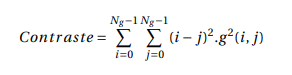
\includegraphics[width=\textwidth]{images/constrate.png}
			\end{minipage}
		\end{center}
	\end{figure}
	
	\item \textbf{Dissimilarité :}
	La dissimilarité quantifie la variation linéaire des niveaux de gris entre des pixels adjacents. Contrairement au contraste, elle pondère les différences de manière linéaire, offrant une autre perspective sur les variations texturales.
	
	\begin{figure}[htbp]
		\begin{center}
			\begin{minipage}[b]{0.5\textwidth}
				\centering
				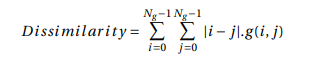
\includegraphics[width=\textwidth]{images/dissimilarity.png}
			\end{minipage}
		\end{center}
	\end{figure}
	
	\item \textbf{Énergie :}
	L'énergie évalue l'uniformité de la texture dans l'image. Une énergie élevée indique une texture homogène et lisse, tandis qu'une énergie faible suggère une texture hétérogène avec de nombreuses variations.
	
	\begin{figure}[H]
		\begin{center}
			\begin{minipage}[b]{0.4\textwidth}
				\centering
				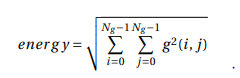
\includegraphics[width=\textwidth]{images/energy.png}
			\end{minipage}
		\end{center}
	\end{figure}
	
	\item \textbf{Homogénéité :}
	L'homogénéité mesure la similarité des niveaux de gris entre les pixels adjacents. Une valeur élevée d'homogénéité signifie une texture uniforme et régulière, tandis qu'une valeur faible indique des variations prononcées.
	
	\begin{figure}[H]
		\begin{center}
			\begin{minipage}[b]{0.5\textwidth}
				\centering
				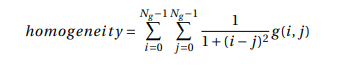
\includegraphics[width=\textwidth]{images/homogenety.png}
			\end{minipage}
		\end{center}
	\end{figure}
	
	\item \textbf{Corrélation :}
	La corrélation évalue la dépendance linéaire des niveaux de gris entre des pixels adjacents. Une corrélation élevée indique une texture régulière et structurée, tandis qu'une corrélation faible révèle des motifs plus aléatoires.
	
	\begin{figure}[H]
		\begin{center}
			\begin{minipage}[b]{0.5\textwidth}
				\centering
				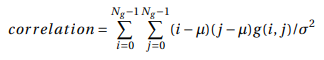
\includegraphics[width=\textwidth]{images/correlation.png}
			\end{minipage}
		\end{center}
	\end{figure}
	
	\item \textbf{Entropie :}
	L'entropie mesure la complexité et la diversité des niveaux de gris dans l'image. Une entropie élevée indique une texture complexe avec de nombreuses variations, tandis qu'une entropie faible suggère une texture plus uniforme et régulière.
	
	\begin{figure}[H]
		\begin{center}
			\begin{minipage}[b]{0.5\textwidth}
				\centering
				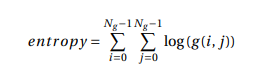
\includegraphics[width=\textwidth]{images/entropy.png}
			\end{minipage}
		\end{center}
	\end{figure}
\end{enumerate}

\subsubsection{Descripteurs des Symptômes des Feuilles}

L'analyse des symptômes sur les feuilles est essentielle pour la détection des maladies du manioc. Les maladies peuvent se manifester par des taches, des décolorations ou des altérations texturales sur les feuilles. En quantifiant ces symptômes, nous pouvons identifier précocement les maladies et prendre des mesures appropriées.

Pour extraire les caractéristiques des symptômes des feuilles, nous suivons les étapes suivantes :
1. Charger l'image en couleurs.
2. Convertir l'image en niveaux de gris.
3. Appliquer un seuillage pour obtenir une image binaire.
4. Trouver les contours des taches dans l'image seuillée.
5. Calculer les caractéristiques des taches telles que le nombre, la surface, la couleur et la texture.

\subsection*{Caractéristiques des Taches}

\subsubsection*{Nombre de Taches}
Le nombre de taches sur une feuille est une caractéristique simple mais informative pour évaluer l'étendue de l'infection.

\[
\text{Nombre de taches} = N_{\text{taches}}
\]

\subsubsection*{Surface des Taches}
La surface totale des taches permet de quantifier l'étendue de la zone affectée par les maladies.

\[
\text{Surface totale des taches} = \sum_{i=1}^{N_{\text{taches}}} A_i
\]

Où \( A_i \) représente la surface de la tache \( i \).

\subsubsection*{Couleur des Taches}
La couleur moyenne des taches est calculée en moyennant les valeurs de couleur dans les régions d'intérêt (ROI) délimitées par les contours des taches.

\[
\text{Couleur moyenne de la tache} = \frac{1}{N_{\text{pixels}}} \sum_{i=1}^{N_{\text{pixels}}} \text{Couleur}(i)
\]

Où \( N_{\text{pixels}} \) est le nombre de pixels dans la région de la tache.

\subsubsection*{Texture des Taches}
La texture des taches, bien que non implémentée dans ce code, pourrait être évaluée en utilisant des descripteurs de texture similaires à ceux utilisés pour la surface des grains de blé, tels que la GLCM.


\begin{enumerate}
	\item \textbf{Surface totale des taches :}
	\[
	\text{Surface totale des taches} = \sum_{i=1}^{N_{\text{taches}}} A_i
	\]
	Où \( A_i \) représente la surface de la tache \( i \).
	
	\item \textbf{Couleur moyenne des taches :}
	\[
	\text{Couleur moyenne de la tache} = \frac{1}{N_{\text{pixels}}} \sum_{i=1}^{N_{\text{pixels}}} \text{Couleur}(i)
	\]
	Où \( N_{\text{pixels}} \) est le nombre de pixels dans la région de la tache.
	
	\item \textbf{Texture des taches :}
	La texture peut être évaluée en utilisant des descripteurs tels que le contraste, la dissimilarité, l'énergie, l'homogénéité et la corrélation. Les formules pour ces descripteurs sont les mêmes que celles utilisées pour les grains de blé et peuvent être appliquées aux régions d'intérêt des taches.
\end{enumerate}


\subsubsection{Analyse des Symptômes des Racines de Manioc}

La détection des symptômes des racines de manioc est essentielle pour identifier les maladies qui affectent cette culture. Parmi ces symptômes, les déformations et les décolorations des racines sont des indicateurs clés de la présence de maladies. Voici les méthodes utilisées pour analyser ces symptômes.

\subsection*{Détection des Déformations des Racines}

Les déformations des racines peuvent indiquer la présence de maladies ou de stress environnemental. Pour détecter ces déformations, nous procédons comme suit :
\begin{enumerate}
	\item Convertir l'image en niveaux de gris pour simplifier l'analyse.
	\item Appliquer un flou gaussien pour réduire le bruit dans l'image.
	\item Utiliser une binarisation adaptative pour obtenir une image binaire.
	\item Trouver les contours des objets dans l'image binarisée.
	\item Calculer la proportion de la zone déformée par rapport à la zone totale de l'image.
\end{enumerate}

\subsubsection*{Formule de la Proportion de la Zone Déformée}
\[
\text{Proportion de la zone déformée} = \frac{\text{Surface des zones déformées}}{\text{Surface totale de l'image}}
\]

\subsection*{Détection des Décolorations des Racines}

Les décolorations des racines sont souvent un signe de maladies. Pour détecter ces décolorations, les étapes suivantes sont suivies :
\begin{enumerate}
	\item Convertir l'image en espace de couleur Lab pour mieux isoler les variations de luminance.
	\item Séparer les canaux de couleur Lab.
	\item Calculer la moyenne et l'écart type du canal L (luminance).
	\item Définir une plage de valeurs pour la luminance basée sur la moyenne et l'écart type.
	\item Créer un masque pour les zones décolorées.
	\item Calculer la proportion de pixels décolorés par rapport à la zone totale.
\end{enumerate}

\subsubsection*{Formule de la Proportion de Pixels Décolorés}
\[
\text{Proportion de pixels décolorés} = \frac{\text{Surface des zones décolorées}}{\text{Surface totale de l'image}}
\]

\subsection*{Caractéristiques des Symptômes des Racines}

Les caractéristiques des symptômes des racines sont regroupées en un ensemble de mesures permettant d'évaluer l'état des racines de manioc.

\begin{itemize}
	\item \textbf{Déformation des racines :} Proportion de la zone déformée par rapport à la zone totale de l'image.
	\item \textbf{Décoloration des racines :} Proportion de pixels décolorés par rapport à la zone totale de l'image.
\end{itemize}

\subsubsection{Analyse des Symptômes des Tiges de Manioc}

La détection des symptômes sur les tiges de manioc, comme les lésions, est cruciale pour identifier les maladies affectant cette culture. Les méthodes suivantes sont utilisées pour analyser ces symptômes.

\subsection*{Détection des Lésions sur les Tiges}

Les lésions sur les tiges peuvent indiquer la présence de maladies ou de stress environnemental. Pour détecter ces lésions, nous procédons comme suit :
\begin{enumerate}
	\item Convertir l'image en niveaux de gris pour simplifier l'analyse.
	\item Appliquer un flou gaussien pour réduire le bruit dans l'image.
	\item Utiliser une binarisation adaptative pour segmenter les lésions.
\end{enumerate}

\subsubsection*{Formule de la Proportion des Lésions}
\[
\text{Proportion de lésions} = \frac{\text{Surface des lésions détectées}}{\text{Surface totale de l'image}}
\]

\subsection*{Mesure de la Longueur et de la Largeur des Lésions}

Pour quantifier les lésions, nous mesurons la longueur et la largeur maximales des lésions détectées :
\begin{enumerate}
	\item Trouver les contours des lésions dans l'image binarisée.
	\item Calculer les dimensions des rectangles englobants pour chaque lésion.
	\item Identifier les dimensions maximales de longueur et de largeur.
\end{enumerate}

\subsubsection*{Formules des Dimensions des Lésions}
\[
\text{Longueur maximale} = \max(\{h_i\})
\]
\[
\text{Largeur maximale} = \max(\{w_i\})
\]
où \( h_i \) et \( w_i \) représentent respectivement la hauteur et la largeur des rectangles englobants des lésions.

\subsection*{Détection de la Couleur des Lésions}

Les changements de couleur sur les tiges peuvent indiquer des lésions. Pour détecter la couleur des lésions, nous procédons comme suit :
\begin{enumerate}
	\item Convertir l'image en espace de couleur HSV (Teinte, Saturation, Valeur).
	\item Appliquer un masque pour isoler les zones de lésions.
	\item Calculer la couleur moyenne des pixels dans les zones de lésions.
\end{enumerate}

\subsubsection*{Formule de la Couleur Moyenne des Lésions}
\[
\text{Couleur moyenne des lésions} = \left( \bar{H}, \bar{S}, \bar{V} \right)
\]
où \( \bar{H} \), \( \bar{S} \) et \( \bar{V} \) représentent respectivement les valeurs moyennes de la teinte, de la saturation et de la valeur dans les zones de lésions.

\subsection*{Caractéristiques des Symptômes des Tiges}

Les caractéristiques des symptômes des tiges sont regroupées en un ensemble de mesures permettant d'évaluer l'état des tiges de manioc.

\begin{itemize}
	\item \textbf{Présence de lésions :} Indique si des lésions sont présentes (\textit{True} ou \textit{False}).
	\item \textbf{Longueur des lésions :} Longueur maximale des lésions détectées.
	\item \textbf{Largeur des lésions :} Largeur maximale des lésions détectées.
	\item \textbf{Couleur des lésions :} Couleur moyenne des lésions en termes de teinte, saturation et valeur.
\end{itemize}

\subsection{Extension de l´Ontologie}

Après avoir décrit chaque descripteur, nous avons pris la décision d'enrichir l'ontologie en ajoutant de nouvelles propriétés et relations afin de la rendre plus utile, complète et capable de représenter de manière précise les connaissances sémantiques du domaine.

Le concept de \textit{dataset} est introduit comme une classe ontologique représentant un ensemble de données regroupées selon certaines caractéristiques communes. Un dataset peut contenir des instances de divers types de données, telles que des images, des textes, des vidéos, etc. Il sert à organiser et structurer ces données, facilitant ainsi leur manipulation et analyse. Dans notre contexte, un dataset regroupe les images des maladies du manioc.

Ce concept de \textit{dataset} peut être associé à des propriétés ontologiques décrivant des informations spécifiques telles que le nom du dataset, sa description, sa source, sa date de création, son format, sa taille, etc. Ces propriétés fournissent des métadonnées sémantiques utiles pour la recherche, la gestion et la compréhension des données.

En outre, les concepts de \textit{contour}, \textit{couleur}, \textit{symptômes} et \textit{texture} sont également intégrés dans l'ontologie. Ces concepts permettent de modéliser sémantiquement les différentes caractéristiques des images utilisées pour détecter les maladies du manioc.

\begin{itemize}
	\item \textbf{Contour} : Représente les frontières des objets ou des zones spécifiques identifiées dans une image. En termes ontologiques, il est associé à des propriétés telles que la forme, la surface, le périmètre, etc.
	
	\item \textbf{Couleur} : Désigne les caractéristiques chromatiques des zones d'intérêt dans les images. Les propriétés sémantiques associées peuvent inclure les valeurs moyennes de teinte, de saturation et de luminosité.
	
	\item \textbf{Symptômes} : Regroupe les manifestations visuelles des maladies du manioc, telles que les taches ou les déformations sur les feuilles et les tiges. Les propriétés incluent la taille, la forme et la distribution des symptômes. Ce concept permet de sémantiquement identifier et caractériser les signes de maladies.
	
	\item \textbf{Texture} : Concerne la surface visuelle des zones d'intérêt dans les images, caractérisée par des descripteurs tels que le contraste, la dissimilarité, l'énergie, l'homogénéité et la corrélation. Ces propriétés sémantiques aident à quantifier les variations texturales dues aux maladies.
\end{itemize}

Nous avons également introduit les concepts suivants, étroitement liés au \textit{dataset} :

\begin{itemize}
	\item \textbf{Définition} : Fournit une description sémantique de la maladie de manioc, incluant ses caractéristiques principales et ses impacts sur les cultures.
	
	\item \textbf{Causes} : Identifie et décrit les facteurs responsables de l'apparition des maladies de manioc, tels que les agents pathogènes, les conditions environnementales, etc.
	
	\item \textbf{Symptômes Globales} : Détaille les signes visuels et physiques associés aux maladies de manioc, permettant une identification précoce et précise.
	
	\item \textbf{Traitement} : Présente les méthodes et pratiques recommandées pour gérer et traiter les maladies de manioc, y compris les interventions chimiques, biologiques et culturales.
	
	\item \textbf{Image} : Lient les images spécifiques contenues dans le dataset aux autres concepts, facilitant ainsi leur utilisation pour la détection, l'analyse et la recherche sur les maladies de manioc.
\end{itemize}

Ces concepts enrichissent l'ontologie en fournissant une modélisation sémantique plus détaillée et une analyse approfondie des images dans le contexte de la détection des maladies du manioc. L'intégration de ces propriétés et relations sémantiques permet une meilleure représentation des connaissances du domaine et améliore la capacité de l'ontologie à répondre aux besoins spécifiques de l'analyse d'image.

\subsubsection*{Figure de la gestion de l'ontologie}

\begin{figure}[H]
	\begin{center}
		\begin{minipage}[b]{1\textwidth}
			\centering
			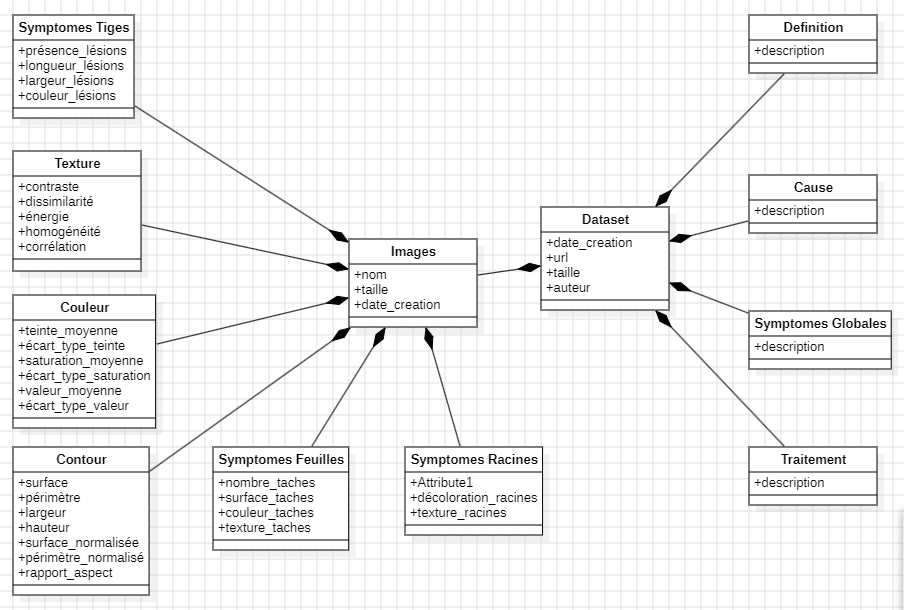
\includegraphics[width=\textwidth]{images/Diagramme.png}
		\end{minipage}
		\caption{Illustre les nouveux concepts ajoutés.}
	\end{center}
\end{figure}

\subsubsection*{Figure de la gestion de l'ontologie dans une base de donnée relationnelle}

\begin{figure}[H]
	\begin{center}
		\begin{minipage}[b]{1\textwidth}
			\centering
			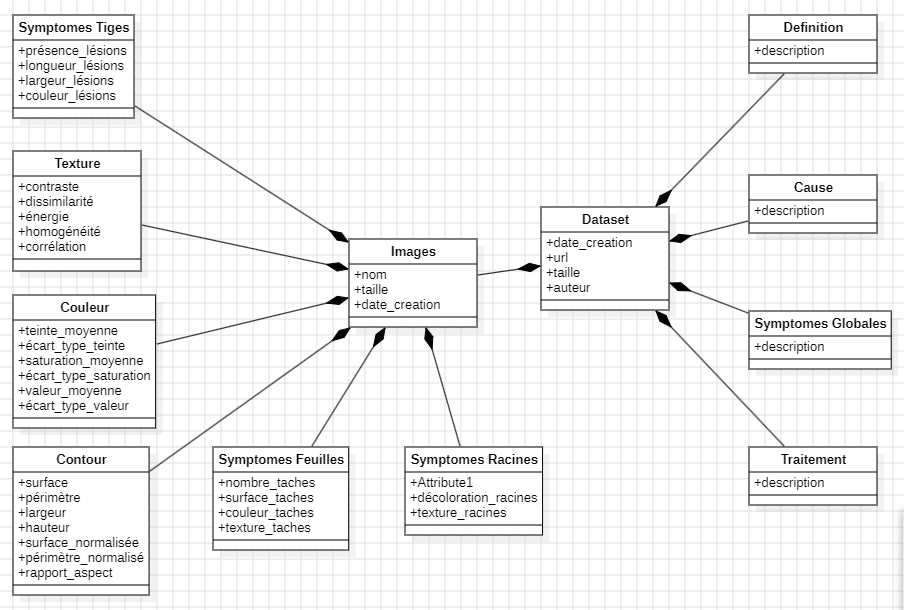
\includegraphics[width=\textwidth]{images/Diagramme.png}
		\end{minipage}
		\caption{Illustre les nouveux concepts ajoutés.}
	\end{center}
\end{figure}

\section{CONCLUSION}
Lorem ipsum dolor sit amet, consectetur adipiscing elit. Sed non risus. Suspendisse lectus tortor, dignissim sit amet, adipiscing nec, ultricies sed, dolor. Cras elementum ultrices diam. Maecenas ligula massa, varius a, semper congue, euismod non, mi. Proin porttitor, orci nec nonummy molestie, enim est eleifend mi, non fermentum diam nisl sit amet erat. Duis semper. Duis arcu massa, scelerisque vitae, consequat in, pretium a, enim. Pellentesque congue. Ut in risus volutpat libero pharetra tempor. Cras vestibulum bibendum augue. Praesent egestas leo in pede. Praesent blandit odio eu enim. Pellentesque sed dui ut augue blandit sodales. Vestibulum ante ipsum primis in faucibus orci luctus et ultrices posuere cubilia Curae; Aliquam nibh. Mauris ac mauris sed pede pellentesque fermentum. Maecenas adipiscing ante non diam sodales hendrerit.